In questo capitolo si utilizza una tecnica basata su rete neurale, ovvero il \textit{Multi-Layer Perceptron}.\\
Mediante scikit-learn è possibile decidere quanti hidden layer inserire e di quali dimensioni. La classe che permette di costruire un MLP è \textit{MLPClassifier}. Inoltre è possibile selezionare il tipo di funzione di attivazione nei neuroni interni:
\begin{itemize}
	\item \textit{identity}: funzione identità $f(x)=x$;
	\item \textit{logistic}: funzione sigmoide tipica della regressione logistica $f(x)=\frac{1}{1+e^{-x}}$
	\item \textit{tanh}: funzione tangente iperbolica $f(x)=\tanh(x)$
	\item \textit{relu}: funzione lineare $f(x)=\max(0,x)$
\end{itemize}
\begin{lstlisting}
from sklearn.neural_network import MLPClassifier

X = brain_tumor_data.drop("Target", axis=1).values
Y = brain_tumor_data["Target"].values
ss = StandardScaler()
X = ss.fit_transform(X)

X_train, X_test, Y_train, Y_test = train_test_split(X, Y, test_size=0.3)

mlp = MLPClassifier(hidden_layer_sizes=(100,), activation='relu', verbose=True, max_iter=300)
mlp.fit(X_train, Y_train)

y_pred_train = mlp.predict(X_train)
y_prob_train = mlp.predict_proba(X_train)

y_pred = mlp.predict(X_test)
y_prob = mlp.predict_proba(X_test)

accuracy_train = accuracy_score(Y_train, y_pred_train)

loss_train = log_loss(Y_train, y_prob_train)

print("ACCURACY: TRAIN=%.4f" % accuracy_train)
print("LOG LOSS: TRAIN=%.4f" % loss_train)
\end{lstlisting}

Il modello adottato è un MLP con un hidden layer formato da 100 neuroni e con funzione di attivazione lineare (relu). I campi \textit{verbose} e \textit{max\_iter} sono utili per la fase di addestramento della rete neurale; il primo è utile per visualizzare in maniera dinamica e testuale la fase di addestramento, mentre il secondo permette di inserire il massimo numero di iterazioni nella fase di addestramento. Sperimentalmente il massimo di 300 iterazioni sono risultati sufficienti per raggiungere l'obiettivo.\\
La fase di addestramento della rete viene iterata finchè non vi sono 10 epoche consecutive dove il loss score non diminuisce di almeno $10^4$. Le metriche calcolate, come nelle altre tecniche, sono l'accuracy e il log loss.\\
\begin{figure}[h]
	\centering   	
	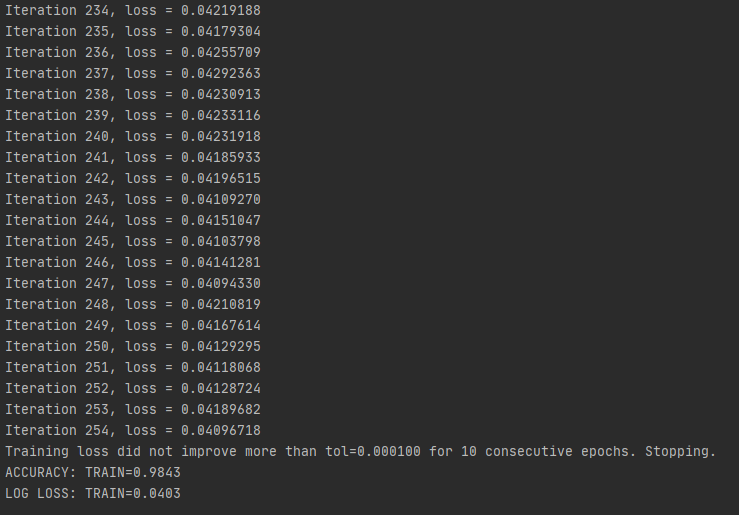
\includegraphics[width=140mm]{image/mlpresults2.png}
	\caption{Fase di addestramento e metriche risultanti.}
\end{figure}
Con questo modello si ha un accuracy pari a circa 0.98 e una log loss di circa 0.04.\\
Un altro tentativo è quello di inserire un ulteriore hidden layer di 100 neuroni sempre con funzione di attivazione lineare. Con tale modello si raggiunge la saturazione dell'addestramento (ovvero le 10 epoche consecutive dove il loss score non diminuisce di almeno $10^4$) molto prima (123 iterazioni) e si raggiunge un accuracy pari a circa 0.99 e una log loss pari a circa 0.03.\\
A questo punto si prova ad aggiungere un ulteriore hidden layer. In questo caso l'addestramento si conclude con 81 iterazioni, ma l'accuracy diminuisce a circa 0.98 e la log loss è pari a circa 0.03.\\
Si prova ora a cambiare la funzione di attivazione settandola come funzione sigmoide. In questo caso, anche con più hidden layer, si ha un accuracy pari a circa a 0.98 e una log loss a circa a 0.05.

\section{Conclusioni su MLP}
In base ai risultati ottenuti, per il dataset a disposizione, il modello con prestazioni migliori è senza dubbio il Multi-Layer Perceptron con due hidden layer di 100 neuroni l'uno e con funzione di attivazione lineare. Una limitazione, non poco importante, è il fatto che la fase di training può occupare molto tempo.